\subsection{Gala prototips}
1. pozīcijā ir HPA un uz viņa novietotie testa lauktranzistori, kas simulē jaudas pastiprinātājus. 2. pozīcijā ir līniju iezīmētie industriālie barošanas avoti. 3. pozīcijā ir monitorēšanas izstrādes plate. 4. pozīcijā ir mikrokontroliera plate. 5. pozīcijā ir RMS jaudas mērītājs. 6. pozīcijā ir pārveidotāju un barošanas avota vadības shēma. 7. pozīcija ir ieslēgšanas/izslēgšanas shēma ar strāvas mērīšanu. 
\begin{figure}[H]
	\centering
    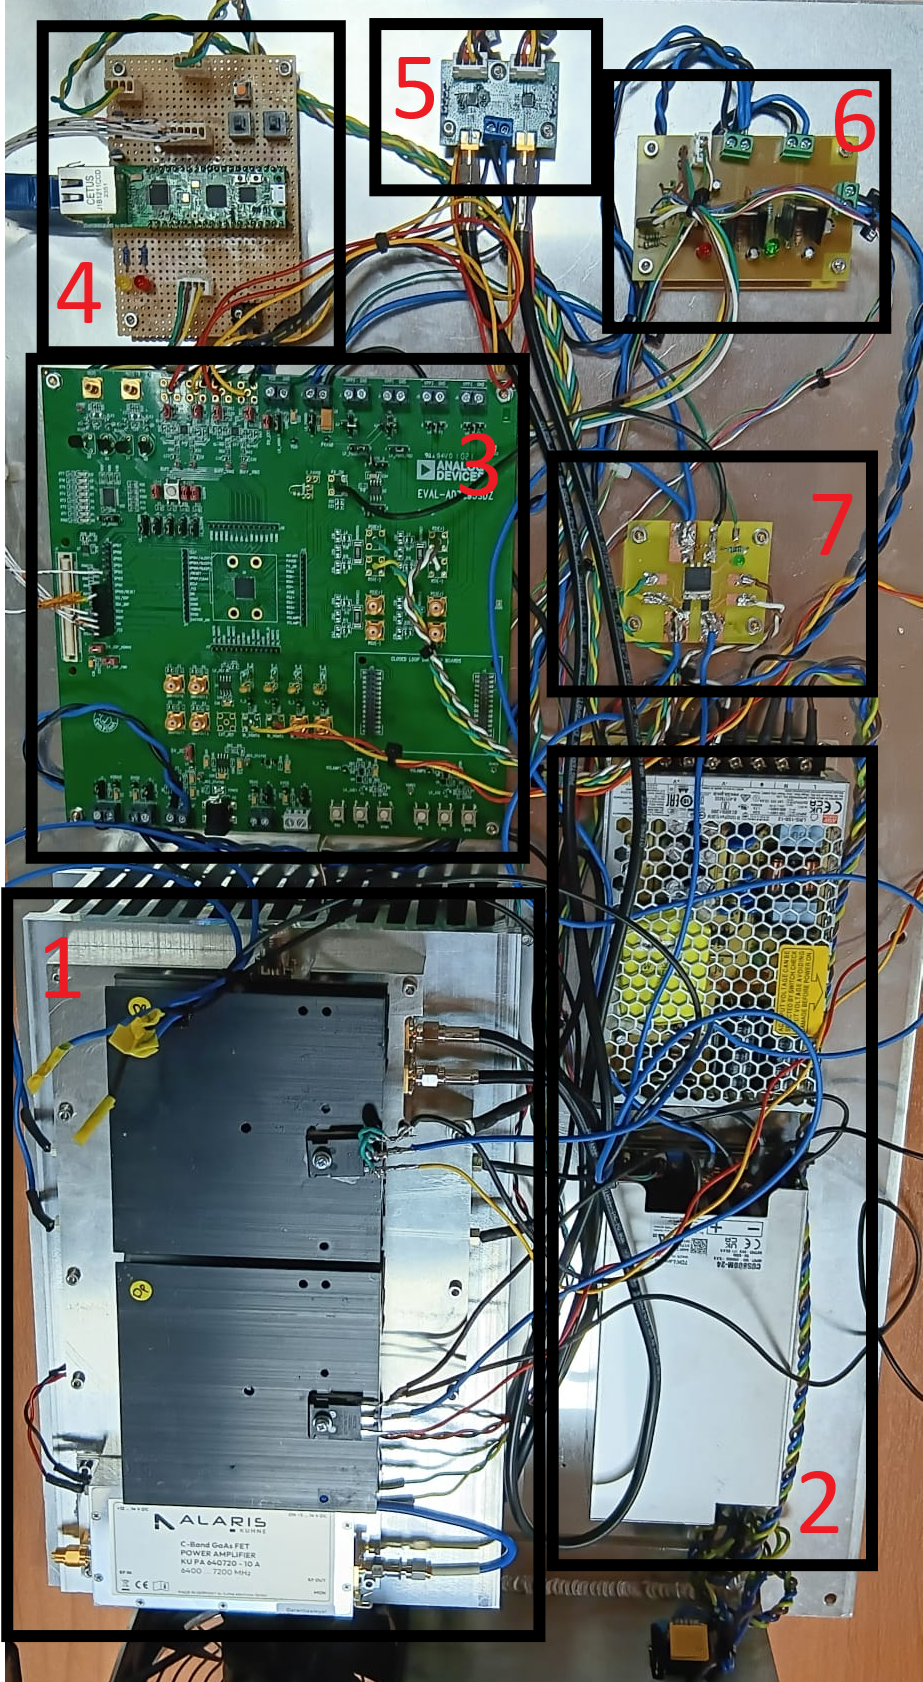
\includegraphics[width=0.9\textwidth]{pictures/finished.png}\hspace{1cm}
    \caption{Prototipa stends}
\end{figure}